\documentclass[tikz,border=3pt]{standalone}
\usepackage[utf8]{inputenc}
\usepackage[T1]{fontenc}
\usepackage{lmodern}
\renewcommand{\familydefault}{\sfdefault}
\usepackage{sansmath}\sansmath
\usepackage{chemfig}
\usepackage{pgfplots}\pgfplotsset{compat=1.18,/pgf/number format/use comma,/pgf/number format/1000 sep={.}}
\usetikzlibrary{arrows.meta,calc,positioning,decorations.pathmorphing,patterns}
% paleta del sitio
\definecolor{nar}{HTML}{E8680C}\definecolor{narc}{HTML}{FFB35C}\definecolor{hielo}{HTML}{FFF3E8}
\definecolor{tinta}{HTML}{1D1D1F}\definecolor{gris}{HTML}{6E6E73}\definecolor{lila}{HTML}{7C5CF0}
\definecolor{azul}{HTML}{2F6FD6}\definecolor{menta}{HTML}{17A673}\definecolor{coral}{HTML}{E8342A}
\begin{document}
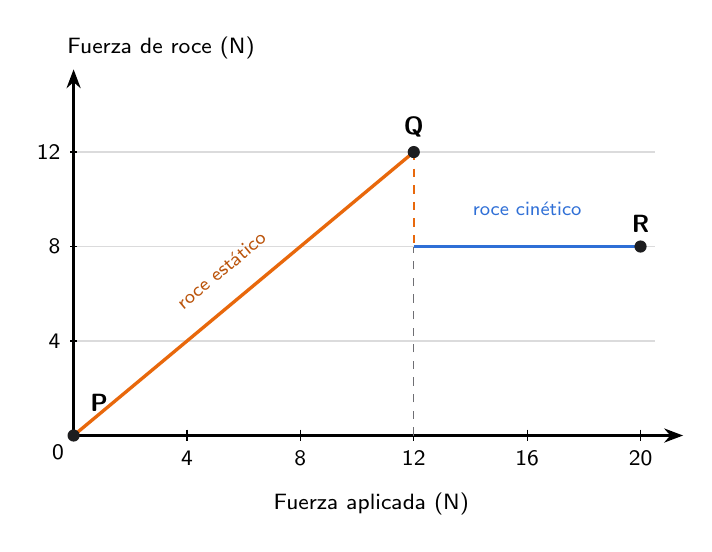
\begin{tikzpicture}[font=\footnotesize,>={Stealth[length=2.4mm]},x=0.36cm,y=0.3cm]
\foreach \y in {4,8,12} \draw[gris!25] (0,\y) -- (20.5,\y);
\draw[->,thick] (0,0) -- (21.5,0);
\node at (10.5,-2.9) {Fuerza aplicada (N)};
\draw[->,thick] (0,0) -- (0,15.5) node[above right=0pt and -6pt] {Fuerza de roce (N)};
\foreach \x in {4,8,...,20} \draw (\x,0.25) -- (\x,-0.25) node[below] {\x};
\foreach \y in {4,8,12} \draw (0.12,\y) -- (-0.12,\y) node[left] {\y};
\node[below left] at (0,0) {0};
\draw[dashed,gris] (12,0) -- (12,8);
\draw[very thick,nar] (0,0) -- (12,12);
\draw[thick,dashed,nar] (12,12) -- (12,8);
\draw[very thick,azul] (12,8) -- (20,8);
\fill[tinta] (0,0) circle (2.2pt) (12,12) circle (2.2pt) (20,8) circle (2.2pt);
\node[font=\small\bfseries] at (0.9,1.4) {P};
\node[font=\small\bfseries,above] at (12,12.2) {Q};
\node[font=\small\bfseries,above] at (20,8.2) {R};
\node[nar!80!black,rotate=39.8,font=\scriptsize] at (5.2,7.0) {roce estático};
\node[azul,font=\scriptsize] at (16,9.6) {roce cinético};
\end{tikzpicture}
\end{document}
